\chapter{Evaluación con editores Blockly existentes}
\label{chap:evaluacion}
\label{chap:casos-evaluacion}

El capítulo anterior explicó cómo se ejecuta e implementa Model2Blockly. Este
capítulo cambia de perspectiva: evalúa hasta qué punto la solución permite
especificar y regenerar editores Blockly que ya existen. La evidencia principal
se construye a partir de diez configuraciones publicadas en los repositorios oficiales de
Blockly. De este modo, la evaluación contrasta la propuesta con editores cuya
estructura no fue creada para ajustarse a las capacidades de Model2Blockly.

La unidad analizada es el \emph{subsistema de edición Blockly}: definiciones de
bloques, campos, entradas, conexiones, paleta y comportamiento del propio
editor. Las aplicaciones seleccionadas incluyen además mapas, lienzos, audio,
animaciones, intérpretes y simuladores. Esas capas consumen el programa construido
con bloques, pero no forman parte del editor generado por Model2Blockly y se
mantienen fuera del alcance. Esta separación es necesaria para no exigir a un
generador de editores que reproduzca también la aplicación específica que los
integra.

El capítulo presenta primero las preguntas de evaluación y el corpus. Después
define los tratamientos, las variables controladas, el descriptor canónico y
las métricas. Las secciones posteriores presentan los resultados funcionales,
el esfuerzo de especificación, los límites observados, la equivalencia entre
las rutas Ecore y \texttt{.m2b}, las amenazas a la validez y la evidencia
técnica complementaria.

\section{Objetivo y preguntas de evaluación}
\label{sec:objetivo-evaluacion}

El objetivo es determinar si Model2Blockly resulta efectivo para crear el
subsistema de edición de editores Blockly existentes y qué esfuerzo de
especificación requiere frente a sus fuentes oficiales. El término
\emph{efectivo} no se identifica únicamente con que una página HTML se abra:
requiere comprobar propiedades observables del editor, registrar las diferencias
y separar las coincidencias de las capacidades todavía no soportadas.

La evaluación responde a cuatro preguntas de investigación, identificadas como
RQ por la expresión inglesa \emph{research question}:

\begin{description}
  \item[RQ1 --- Reproducción funcional.] ¿Qué proporción de las propiedades
  observables de los diez editores puede reproducirse mediante Model2Blockly?

  \item[RQ2 --- Esfuerzo de especificación.] ¿Cómo cambia el tamaño de la
  fuente que debe mantener el desarrollador frente a la implementación oficial
  mediante las APIs JSON o JavaScript de Blockly?

  \item[RQ3 --- Límites.] ¿Qué características de los editores oficiales no
  pueden expresarse, o solo pueden expresarse parcialmente, con el metamodelo,
  el DSL y el generador actuales?

  \item[RQ4 --- Rutas de entrada.] Para una muestra simple, una intermedia y
  una compleja, ¿las rutas Ecore y \texttt{.m2b} producen el mismo descriptor
  canónico de editor?
\end{description}

RQ1 (reproducción funcional) y RQ3 (límites) evalúan la cobertura observable;
RQ2 (esfuerzo de especificación) compara artefactos mantenidos y repetibles;
RQ4 (rutas de entrada) comprueba la coherencia interna de las dos entradas. No se mide
tiempo de desarrollo, porque los modelos fueron construidos durante el propio
desarrollo de la investigación y ese tiempo no constituiría un experimento
humano controlado. Tampoco se evalúan aprendizaje o usabilidad con usuarios
finales.

\section{Corpus de editores existentes}
\label{sec:corpus-evaluacion}

El corpus reúne las ocho aplicaciones enumeradas en el catálogo oficial de
Blockly Games ---Puzzle, Maze, Bird, Turtle, Movie, Music, Pond Tutor y Pond---
y dos demostraciones del repositorio oficial \texttt{blockly-samples}: Graph
Demo y JS-Interpreter Wait
\cite{blocklyGamesCatalogue,blocklyGamesRepository,blocklySamplesRepository}.
La selección es intencional: cubre desde un único bloque hasta editores con
paletas, campos personalizados, mutadores (\emph{mutators}), configuración inicial y decenas de
tipos. No se presenta como muestra aleatoria de todos los editores construidos
con Blockly.

Varias aplicaciones modifican su paleta según el nivel. En esos casos se fija
la configuración que expone el conjunto más completo y estable de capacidades
sin cambiar de modalidad de editor. Pond Tutor usa el nivel 9 porque los niveles
impares muestran Blockly y ese es el último de dicha modalidad. Puzzle no
emplea una paleta convencional y se evalúa mediante su espacio de trabajo
inicial. La Tabla \ref{tab:corpus-blockly} resume las diez unidades concretas.

\begin{table}[htbp]
  \centering
  \scriptsize
  \setlength{\tabcolsep}{3.5pt}
  \begin{tabular}{@{}
      L{0.13\textwidth}
      L{0.19\textwidth}
      L{0.36\textwidth}
      L{0.12\textwidth}
      >{\raggedleft\arraybackslash}p{0.08\textwidth}@{}}
    \toprule
    Caso & Editor & Configuración fijada & Complejidad & Bloques \\
    \midrule
    E01 & Graph Demo & Demostración completa. & Simple & 2 \\
    E02 & JS-Interpreter Wait & Demostración asíncrona con
      \texttt{wait\_seconds}. & Simple & 1 \\
    E03 & Maze & Nivel 10, paleta máxima y estable. & Media & 5 \\
    E04 & Bird & Nivel 10, paleta máxima. & Media & 8 \\
    E05 & Movie & Nivel 10, editor libre. & Media & 5 \\
    E06 & Music & Nivel 10, paleta completa. & Compleja & 6 \\
    E07 & Turtle & Nivel 10, editor libre. & Compleja & 12 \\
    E08 & Puzzle & Espacio de trabajo inicial, sin paleta convencional.
      & Compleja & 3 \\
    E09 & Pond Tutor & Nivel 9, última configuración Blockly del tutor.
      & Compleja & 11 \\
    E10 & Pond & Editor completo de Pond Duck. & Compleja & 24 \\
    \bottomrule
  \end{tabular}
  \caption{Corpus de configuraciones oficiales usado en la evaluación}
  \label{tab:corpus-blockly}
\end{table}

Para preservar la reproducibilidad, las fuentes no se obtienen de la versión
más reciente en cada ejecución. Blockly Games se fija en la revisión identificada
por \texttt{5d2ff6f39207} y \texttt{blockly-samples} en
\texttt{62ce12097707}; los hashes completos se conservan en el manifiesto del
experimento. Cada fragmento extraído
registra repositorio, ruta, intervalo de líneas y hash SHA-256. Esto permite
verificar que la referencia comparada es la misma aunque las ramas principales
de los proyectos evolucionen.

\section{Unidad de análisis y alcance}
\label{sec:alcance-evaluacion-externa}

La evaluación distingue tres capas para cada aplicación:

\begin{enumerate}
  \item \textbf{editor Blockly}: tipos de bloque, textos, campos, entradas,
  conexiones, colores, ayudas, paleta, configuración inicial y comportamiento
  dinámico que modifica la edición;
  \item \textbf{generación de código}: presencia y estructura declarativa de
  los generadores asociados a los bloques, informada por separado;
  \item \textbf{aplicación de dominio}: interpretación, simulación, mapas,
  lienzos, audio, animaciones, puntuación y navegación exterior al editor.
\end{enumerate}

La primera capa constituye la métrica principal de RQ1 (reproducción
funcional). La segunda se separa
para no considerar que una forma de bloque correcta demuestra también la
ejecución completa de su código. La tercera se excluye. Por ejemplo, en Maze se
comparan los cinco bloques y la paleta del nivel 10, pero no el mapa ni la
animación de Pegman; en Turtle se comparan los bloques de dibujo, pero no el
lienzo que interpreta sus instrucciones; en Music no se reproduce el motor de
audio.

También debe distinguirse el motor de renderizado (\emph{renderer}) de Blockly
de la visualización del dominio. Geras o Zelos son motores internos de
renderizado que determinan cómo Blockly dibuja
la geometría de los bloques. El mapa de Maze o el lienzo de Turtle son capas de
la aplicación anfitriona. En el experimento se fija Geras como variable de
control, mientras que las visualizaciones de dominio quedan excluidas.

Dentro del editor se incluyen identificadores, orden visible, clases y valores
de campos, comprobaciones de tipo, conexiones, disposición, color, texto
emergente de ayuda, enlace de ayuda, categorías, entradas de la paleta, sombras,
valores preconfigurados,
mutadores, validadores y cambios dinámicos de forma. Una capacidad incluida no
se retira del denominador cuando Model2Blockly no puede expresarla: se registra
como diferencia y contribuye a RQ3 (límites de la solución).

\section{Diseño experimental}
\label{sec:diseno-experimental-blockly}

\subsection{Tratamientos y variables controladas}

Para cada caso se construyen dos tratamientos:

\begin{itemize}
  \item \textbf{BASELINE}: fragmentos sin modificar de la definición oficial
  del subsistema de edición;
  \item \textbf{M2B}: modelo \texttt{.m2b} mantenido para el caso y editor
  producido por la cadena real de Model2Blockly.
\end{itemize}

Ambos tratamientos se cargan en el mismo contenedor de prueba con Blockly
13.1.1, renderizador Geras, tema Classic, configuración regional inglesa, ventana de
1280~$\times$~800 píxeles y espacio de trabajo de 1024~$\times$~640 píxeles. Las
dependencias se instalan localmente y no se obtiene una versión variable desde
una CDN. Cuando una fuente antigua requiere compatibilidad con Blockly 13.1.1,
la adaptación se mantiene en un fichero independiente, se documenta y se
excluye del cómputo de código oficial.

Graph, Maze y Turtle incorporan además un tratamiento \textbf{ECORE}. Los tres
representan, respectivamente, complejidad simple, media y compleja. Su función
es responder RQ4 (rutas de entrada): ECORE y M2B describen el mismo editor y sus resultados se
comparan entre sí; ECORE no sustituye al BASELINE oficial.

La Figura \ref{fig:flujo-evaluacion-externa} resume el flujo. La comparación
principal enfrenta el descriptor oficial con el descriptor generado desde
\texttt{.m2b}. La comprobación Ecore es una comparación emparejada adicional
sobre tres casos y no altera las métricas de los diez editores.

\begin{figure}[htbp]
  \centering
  \resizebox{0.98\textwidth}{!}{%
  \begin{tikzpicture}[
      node distance=0.55cm and 0.85cm,
      source/.style={draw=black!55, rounded corners=2pt, fill=green!8,
        minimum width=3.1cm, minimum height=0.75cm, align=center, font=\small},
      process/.style={draw=black!55, rounded corners=2pt, fill=blue!7,
        minimum width=3.2cm, minimum height=0.75cm, align=center, font=\small},
      result/.style={draw=black!55, rounded corners=2pt, fill=orange!10,
        minimum width=3.25cm, minimum height=0.75cm, align=center, font=\small},
      arrow/.style={-{Latex[length=2.4mm]}, thick, draw=black!70}
    ]
    \node[source] (official) {Fuente oficial\\BASELINE};
    \node[source, below=of official] (m2b) {Modelo del caso\\\texttt{.m2b}};
    \node[source, below=of m2b] (ecore) {Modelo equivalente\\Ecore (E01, E03, E07)};

    \node[process, right=of official] (officialHarness)
      {Contenedor Blockly\\controlado};
    \node[process, right=of m2b] (m2bGeneration)
      {Generación Model2Blockly\\+ contenedor controlado};
    \node[process, right=of ecore] (ecoreGeneration)
      {Generación Model2Blockly\\+ contenedor controlado};

    \node[result, right=of officialHarness] (officialDescriptor)
      {Descriptor canónico\\oficial};
    \node[result, right=of m2bGeneration] (m2bDescriptor)
      {Descriptor canónico\\M2B};
    \node[result, right=of ecoreGeneration] (ecoreDescriptor)
      {Descriptor canónico\\Ecore};

    \node[result, right=1.05cm of m2bDescriptor] (comparison)
      {Comparación\\de resultados};

    \draw[arrow] (official) -- (officialHarness);
    \draw[arrow] (m2b) -- (m2bGeneration);
    \draw[arrow] (ecore) -- (ecoreGeneration);
    \draw[arrow] (officialHarness) -- (officialDescriptor);
    \draw[arrow] (m2bGeneration) -- (m2bDescriptor);
    \draw[arrow] (ecoreGeneration) -- (ecoreDescriptor);
    \draw[arrow] (officialDescriptor.east) -- ++(0.42,0) |- (comparison.north);
    \draw[arrow] (m2bDescriptor) -- (comparison);
    \draw[arrow] (ecoreDescriptor.east) -- ++(0.42,0) |- (comparison.south);
  \end{tikzpicture}%
  }
  \caption{Tratamientos y comparaciones de la evaluación externa}
  \label{fig:flujo-evaluacion-externa}
\end{figure}

\subsection{Descriptor canónico y regla de comparación}

El contenedor transforma cada tratamiento en un descriptor JSON independiente
de su sintaxis de origen. El descriptor registra los controles de ejecución,
los bloques, la paleta, el espacio inicial, los generadores y los errores de
carga. Cada bloque se descompone en propiedades atómicas: orden de entradas,
campos, comprobaciones, conexiones, disposición, color, texto emergente de ayuda,
enlace de ayuda y comportamiento dinámico. El orden de las propiedades JSON es irrelevante, pero
se conserva el orden visible de campos, entradas, categorías y elementos de la
paleta.

Cada propiedad observada recibe uno de estos estados:

\begin{itemize}
  \item \texttt{match}: valor y comportamiento observable equivalentes;
  \item \texttt{partial}: aproximación de la misma capacidad con una diferencia
  concreta documentada;
  \item \texttt{mismatch}: la capacidad existe, pero el valor generado no
  coincide;
  \item \texttt{unsupported}: la representación no existe en la cadena actual;
  \item \texttt{error}: el bloque o el editor generado no puede cargarse;
  \item \texttt{excluded}: diferencia observada que pertenece a la capa de
  ejecución excluida y no entra en el denominador.
\end{itemize}

Toda propiedad inicialmente distinta debe corresponder con una única regla de
evaluación que indique capacidad, límite afectado y justificación. Una
diferencia sin regla, dos reglas aplicables a la misma propiedad o una regla que
ya no corresponde con el resultado hacen fallar la verificación. Esta condición
evita reclasificar de forma silenciosa una diferencia para favorecer la cifra
final.

La métrica principal de RQ1 (reproducción funcional) es:

\begin{equation}
  \text{paridad del editor} =
  \frac{\text{propiedades \texttt{match}}}
       {\text{propiedades aplicables}} \times 100.
  \label{eq:paridad-editor}
\end{equation}

El denominador incluye \texttt{match}, \texttt{partial}, \texttt{mismatch},
\texttt{unsupported} y \texttt{error}. Las diferencias \texttt{excluded} se
publican por separado. Un caso se clasifica como \emph{completo} cuando alcanza
el 100\,\% sin errores; \emph{parcial} cuando carga, pero conserva alguna
diferencia; y \emph{no reproducible} cuando el editor o sus bloques principales
no pueden cargarse. Los generadores utilizan los mismos estados, aunque su
paridad se informa fuera de la puntuación principal del editor.

\subsection{Métrica de esfuerzo de especificación}

RQ2 (esfuerzo de especificación) compara la fuente mantenida, no la salida
generada. En BASELINE se cuentan
solo las definiciones, extensiones del editor, construcción de la paleta y
generadores necesarios para la configuración. Se excluyen licencias, importaciones,
HTML contenedor, traducciones, motores de dominio y bibliotecas. En M2B se cuenta
el fichero \texttt{source.m2b}; los JavaScript y HTML generados no entran en la
medida.

Para ambos tratamientos se registran bytes UTF-8, líneas totales, líneas no
vacías y líneas no vacías sin comentarios. La comparación principal utiliza
esta última unidad:

\begin{equation}
  \text{reducción LOC} =
  \left(1 - \frac{\text{LOC}_{\mathrm{m2b}}}
                    {\text{LOC}_{\mathrm{oficial}}}\right) \times 100.
  \label{eq:reduccion-loc}
\end{equation}

Se ofrecen valores por caso, media, mediana y total ponderado. Pond Tutor y Pond
reutilizan líneas de los mismos ficheros oficiales. Por ello, además de sumar
las diez configuraciones como artefactos independientes, se calcula un total
conservador que elimina una línea oficial solo cuando coinciden repositorio,
revisión, ruta y número de línea. Los diez modelos \texttt{.m2b} se conservan en
ese cálculo porque se mantienen como especificaciones independientes.

Ecore se excluye deliberadamente de esta métrica. Comparar LOC de XML/XMI con
las del DSL mezclaría unidades de edición distintas. En RQ4 (rutas de entrada), los descriptores de
Ecore y \texttt{.m2b} deben ser estrictamente iguales en controles, bloques,
paleta, espacio inicial, generadores, errores y capacidad de carga; el resultado
es equivalencia o no equivalencia, acompañado de las diferencias si las hubiera.

\section{Procedimiento y reproducibilidad}
\label{sec:procedimiento-evaluacion-blockly}

Cada caso sigue el mismo procedimiento:

\begin{enumerate}
  \item fijar repositorio, revisión y configuración concreta;
  \item identificar los fragmentos oficiales incluidos en el alcance;
  \item extraerlos sin modificación y verificar intervalos y hashes;
  \item escribir el modelo \texttt{.m2b} del editor;
  \item ejecutar la cadena real de generación;
  \item cargar BASELINE y M2B bajo los mismos controles de navegador;
  \item instanciar los bloques y obtener los descriptores canónicos;
  \item comparar sus propiedades y exigir una justificación única para cada
  diferencia;
  \item recopilar LOC y bytes con el mismo programa de medición;
  \item conservar resultados JSON y capturas como evidencia reproducible.
\end{enumerate}

Las capturas permiten inspeccionar que los tratamientos se cargan y presentan
los bloques esperados, pero no se usan como prueba de equivalencia píxel a
píxel. La decisión se basa en propiedades estructurales y en errores observados
por el navegador. En E01, E03 y E07 se añade después la generación Ecore y se
exige igualdad exacta con el descriptor M2B.

El corpus, los controles y las revisiones se declaran en el manifiesto
\path{evaluation/official-blockly/}\allowbreak\path{manifest.json}. Cada directorio de caso
contiene la extracción oficial, \path{source.m2b}, la salida generada, las
reglas de evaluación, los descriptores, las métricas y las capturas. La orden
\texttt{npm run verify:evaluation-completed} ejecuta el contenedor y los diez
casos; \texttt{npm run aggregate:evaluation} regenera el resumen global. Los
resultados individuales se conservan para que la media no oculte un caso y para
que cada limitación pueda rastrearse hasta una propiedad concreta.

La construcción de los dos primeros casos, Graph y Maze, se utilizó como piloto
para fijar el esquema del descriptor, el emparejamiento de campos y los estados
de comparación antes de completar el corpus. Una vez fijados, esos criterios se
aplicaron sin cambiar su granularidad a los ocho casos restantes. La siguiente
sección presenta los resultados obtenidos mediante este protocolo.

\section{Resultados de la reproducción funcional}
\label{sec:resultados-reproduccion}

La Tabla~\ref{tab:resultados-casos-blockly} reúne los resultados por caso. La
columna de editor mide las propiedades estructurales de los bloques y de la
paleta; la columna de generadores mide las propiedades de generación que forman
parte del alcance. En ambas se muestra el número de coincidencias sobre las
propiedades aplicables. Las diferencias excluidas del alcance no aparecen en el
denominador. Las tres últimas columnas comparan las LOC de configuración
oficiales con las LOC del modelo \texttt{.m2b}.

\begin{table}[htbp]
  \centering
  \caption{Resultados por caso: paridad funcional y esfuerzo de especificación}
  \label{tab:resultados-casos-blockly}
  \resizebox{\textwidth}{!}{%
  \begin{tabular}{llrrrrrrrr}
    \toprule
    Caso & Editor & Bloques & Editor $m/a$ & Editor (\%) & Gen. $m/a$ & Gen. (\%) & LOC oficial & LOC M2B & Red. (\%) \\
    \midrule
    E01 & Graph       &  2 &  77/91  & 84,62 &  7/8   & 87,50 & 329 &  28 & 91,49 \\
    E02 & Wait        &  1 &  73/89  & 82,02 &  4/4   & 100,00 & 282 &  16 & 94,33 \\
    E03 & Maze        &  5 & 111/137 & 81,02 & 15/15  & 100,00 & 178 &  73 & 58,99 \\
    E04 & Bird        &  8 & 203/218 & 93,12 & 27/31  & 87,10 & 246 &  93 & 62,20 \\
    E05 & Movie       &  5 & 236/283 & 83,39 & 16/20  & 80,00 & 449 &  75 & 83,30 \\
    E06 & Music       &  6 & 186/232 & 80,17 & 19/21  & 90,48 & 545 &  94 & 82,75 \\
    E07 & Turtle      & 12 & 349/427 & 81,73 & 30/40  & 75,00 & 669 & 190 & 71,60 \\
    E08 & Puzzle      &  3 &  59/75  & 78,67 &  6/12  & 50,00 & 221 &  46 & 79,19 \\
    E09 & Pond Tutor  & 11 & 340/397 & 85,64 & 35/44  & 79,55 & 415 & 154 & 62,89 \\
    E10 & Pond        & 24 & 681/813 & 83,76 & 68/96  & 70,83 & 740 & 352 & 52,43 \\
    \midrule
    Total & & 77 & 2315/2762 & 83,82 & 227/291 & 78,01 & 4074 & 1121 & 72,48 \\
    \bottomrule
  \end{tabular}%
  }
\end{table}

En el editor se obtienen 2315 coincidencias entre 2762 propiedades aplicables,
lo que corresponde a una paridad ponderada del 83,82\,\%. La media no ponderada
por caso es 83,41\,\% y la mediana 82,71\,\%. El intervalo va desde el 78,67\,\%
de Puzzle hasta el 93,12\,\% de Bird. Los veinte tratamientos BASELINE/M2B se
cargaron sin errores y todos los bloques declarados por los modelos pudieron
instanciarse. No obstante, ninguno de los diez casos alcanza el 100\,\%: los
diez se clasifican como reproducciones \emph{parciales}, y no como equivalencias
completas.

La distribución agregada de estados, mostrada en la
Tabla~\ref{tab:estados-agregados}, hace visible lo que una sola puntuación
ocultaría. En particular, 366 propiedades del editor y 50 de los generadores no
pueden expresarse todavía mediante la especificación común. Los ocho
\texttt{mismatch} del editor corresponden a redefiniciones de bloques reservados;
los seis de los generadores se concentran en la serialización automática de
Puzzle.

\begin{table}[htbp]
  \centering
  \caption{Distribución agregada de estados de comparación}
  \label{tab:estados-agregados}
  \begin{tabular}{lrr}
    \toprule
    Estado & Editor & Generadores \\
    \midrule
    \texttt{match}       & 2315 & 227 \\
    \texttt{partial}     &   73 &   8 \\
    \texttt{mismatch}    &    8 &   6 \\
    \texttt{unsupported} &  366 &  50 \\
    \texttt{error}       &    0 &   0 \\
    \texttt{excluded}    &    0 &  17 \\
    \bottomrule
  \end{tabular}
\end{table}

La Figura~\ref{fig:evidencia-visual-corpus} presenta dos pares representativos:
Maze, de complejidad media, y Pond, el caso mayor del corpus. Las capturas
confirman que ambos tratamientos cargan una paleta y un espacio de trabajo
comparables. Sin embargo, no sustituyen a la comparación estructural: dos
capturas visualmente próximas pueden ocultar diferencias en conexiones,
valores internos de campos o generadores.

\begin{figure}[p]
  \centering
  \begin{minipage}{0.48\textwidth}
    \centering
    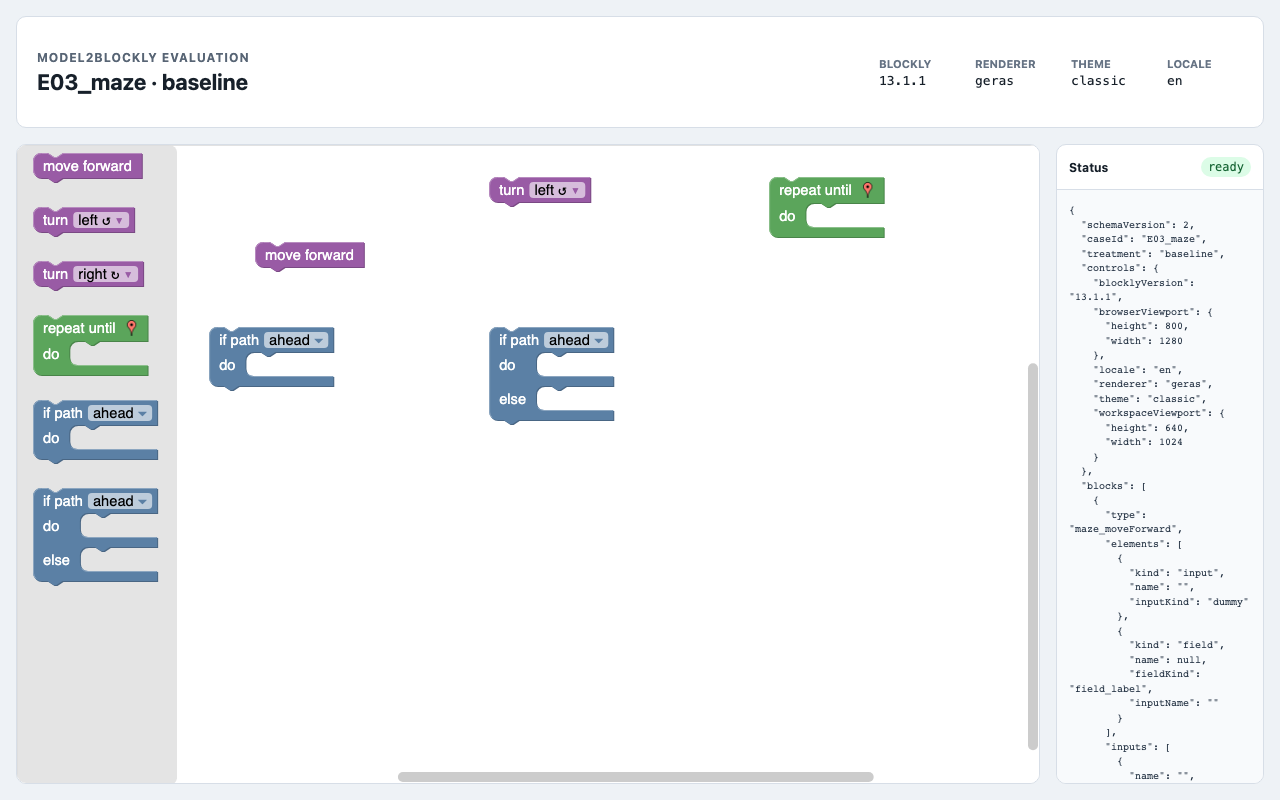
\includegraphics[width=\linewidth]{../../evaluation/official-blockly/cases/E03_maze/results/screenshots/baseline.png}
    \\[2pt]\small (a) Maze oficial
  \end{minipage}\hfill
  \begin{minipage}{0.48\textwidth}
    \centering
    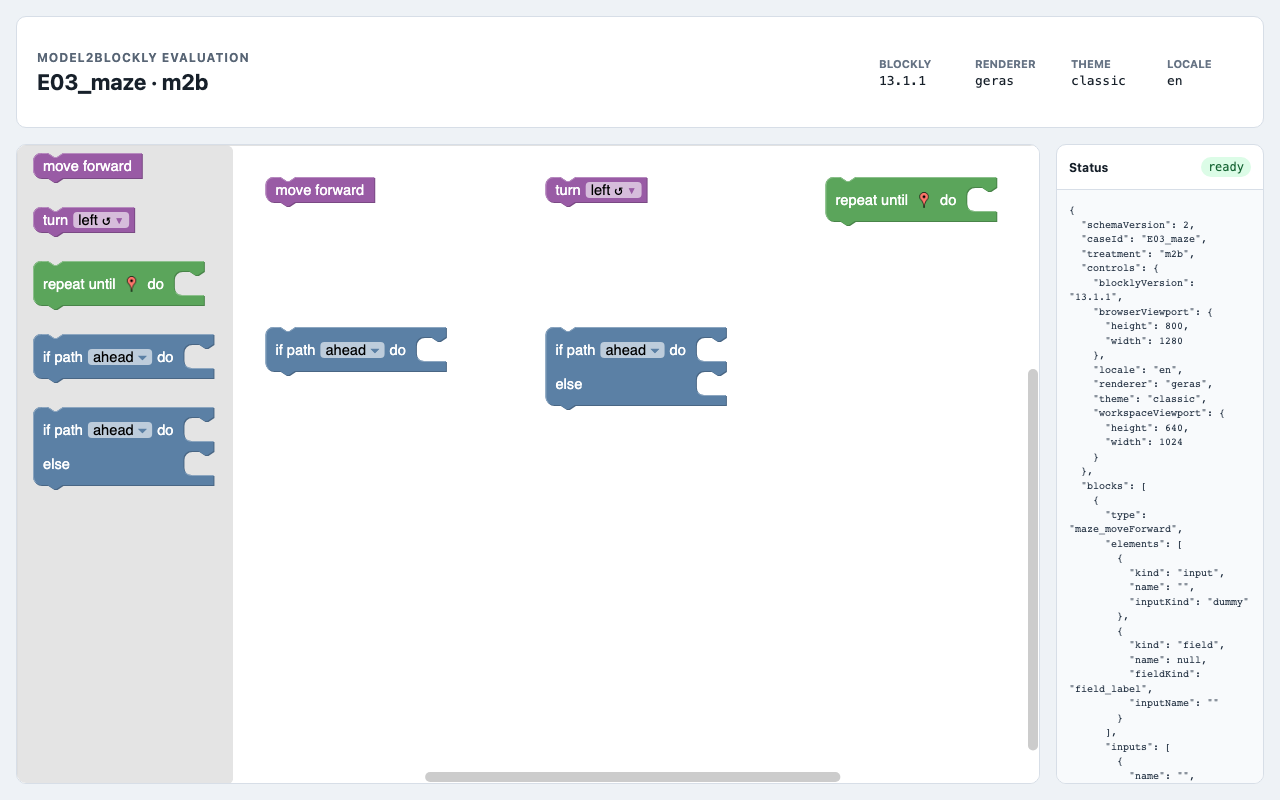
\includegraphics[width=\linewidth]{../../evaluation/official-blockly/cases/E03_maze/results/screenshots/m2b.png}
    \\[2pt]\small (b) Maze generado con M2B
  \end{minipage}

  \vspace{0.8em}

  \begin{minipage}{0.48\textwidth}
    \centering
    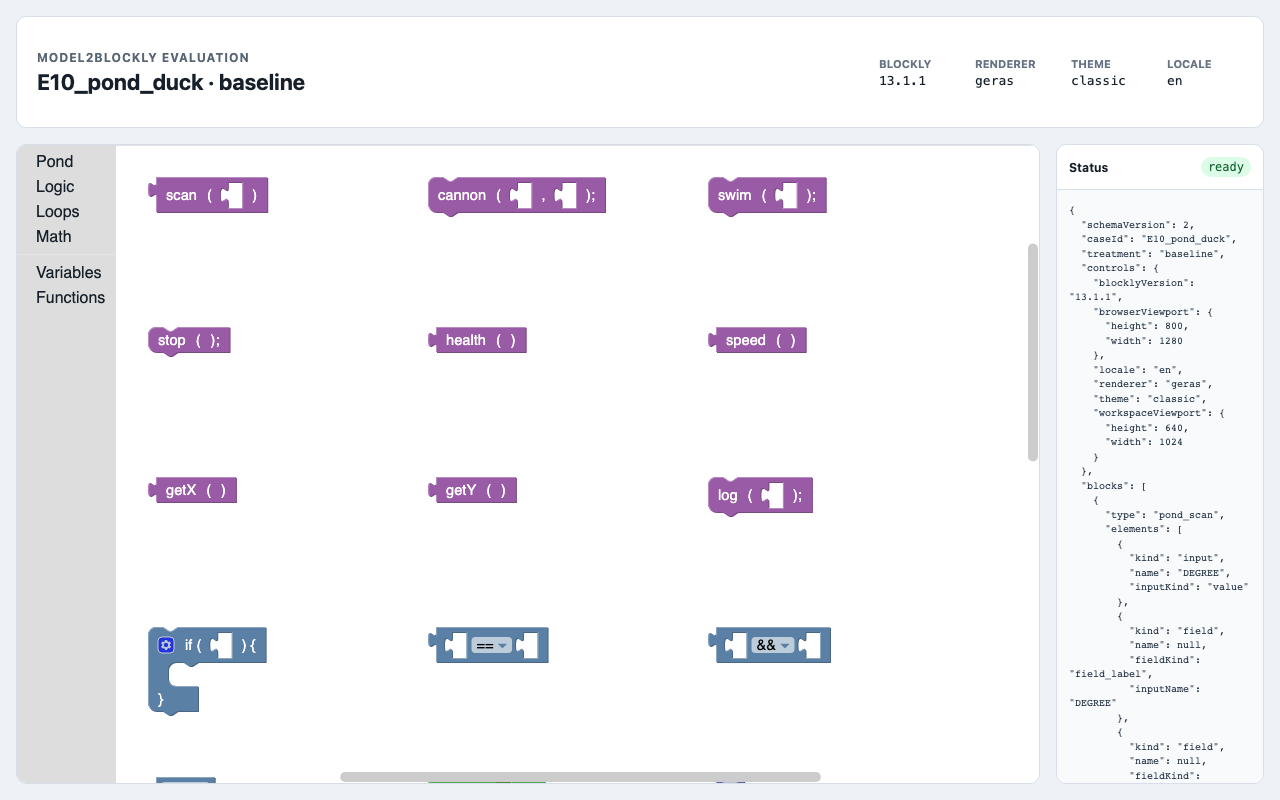
\includegraphics[width=\linewidth]{../../evaluation/official-blockly/cases/E10_pond_duck/results/screenshots/baseline.png}
    \\[2pt]\small (c) Pond oficial
  \end{minipage}\hfill
  \begin{minipage}{0.48\textwidth}
    \centering
    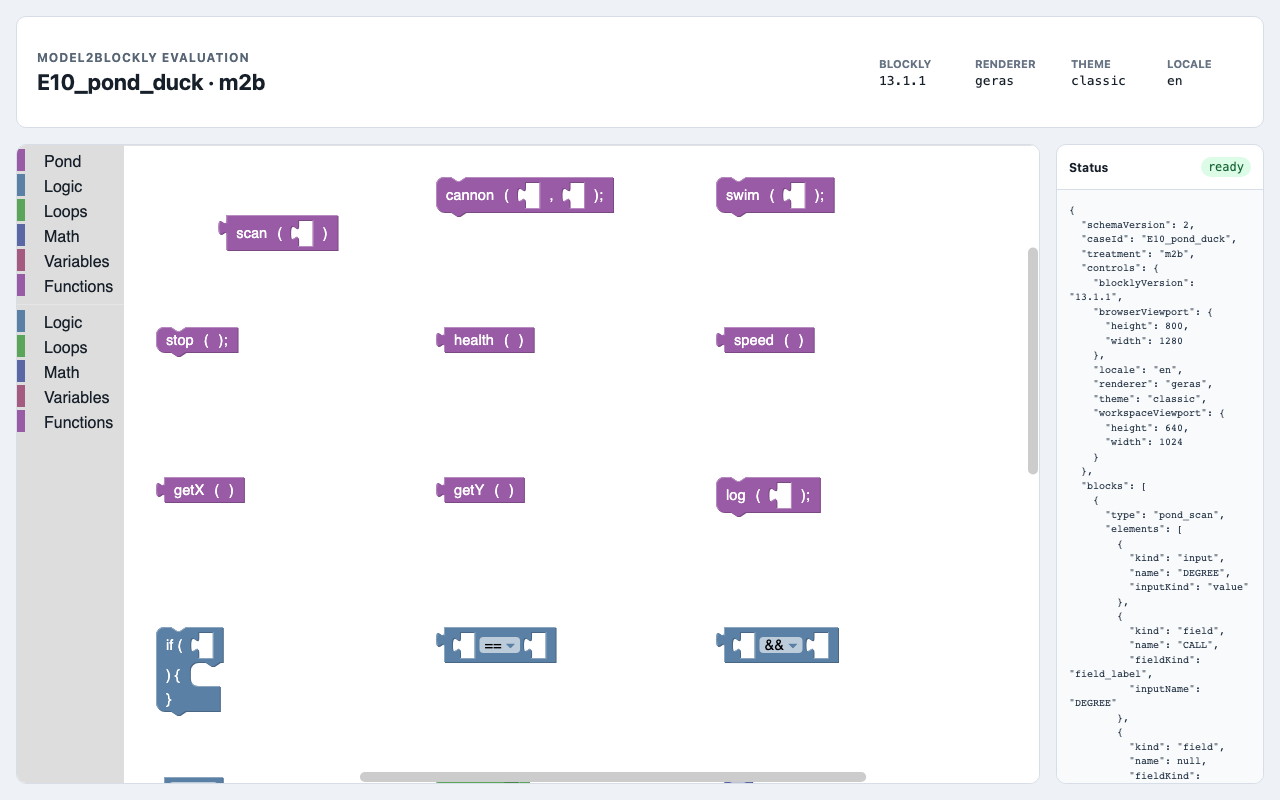
\includegraphics[width=\linewidth]{../../evaluation/official-blockly/cases/E10_pond_duck/results/screenshots/m2b.png}
    \\[2pt]\small (d) Pond generado con M2B
  \end{minipage}
  \caption{Evidencia visual auxiliar de dos casos del corpus}
  \label{fig:evidencia-visual-corpus}
\end{figure}

\subsection{Resultados de los generadores}

La paridad ponderada de los generadores es 227/291, es decir, 78,01\,\%. La
media por caso es 82,05\,\% y la mediana 83,55\,\%. Diecisiete propiedades se
marcaron como \texttt{excluded}: pertenecen al seguimiento de ejecución y a los
mecanismos de interrupción de bucles de Blockly Games, que instrumentan el
programa para la aplicación educativa, pero no definen el editor ni la
traducción básica de cada bloque.

Los resultados de Wait y Maze alcanzan el 100\,\% dentro del alcance, mientras
que Puzzle obtiene el 50\,\%. La causa principal de este último valor es que el
caso oficial serializa automáticamente el estado completo del rompecabezas,
mientras que Model2Blockly genera funciones asociadas a tipos de bloque. En los
casos Pond aparecen además procedimientos, variables y mutadores, que requieren
estado compartido durante la generación. Por tanto, la menor puntuación de esta
capa no implica que el editor no cargue; indica que la semántica de generación
oficial no siempre puede reconstruirse con el contrato actual.

\section{Resultados del esfuerzo de especificación}
\label{sec:resultados-esfuerzo}

Las diez configuraciones oficiales suman 4074 LOC no vacías y sin comentarios,
frente a 1121 LOC de los modelos \texttt{.m2b}. Aplicando la
Ecuación~\ref{eq:reduccion-loc}, la reducción ponderada es 72,48\,\%. La media de
las reducciones individuales es 73,92\,\% y la mediana 75,40\,\%. En bytes UTF-8
la reducción es semejante: de 137358 a 40563 bytes, un 70,47\,\%.

El total anterior considera cada editor como un artefacto mantenible
independiente. Para evitar que la reutilización oficial entre Pond Tutor y Pond
favorezca artificialmente a M2B, se repitió el cómputo eliminando las líneas
oficiales compartidas. El total oficial conservador pasa a 3737 LOC y la
reducción se mantiene en 70,00\,\% (67,67\,\% en bytes). Por tanto, la tendencia
no depende de contar dos veces las 337 líneas comunes.

El resultado debe interpretarse junto con la paridad funcional. Model2Blockly
reduce de forma sustancial el tamaño de la fuente mantenida, pero los modelos no
son sustitutos exactos de todas las configuraciones oficiales. El corpus
demuestra simultáneamente una reducción de esfuerzo descriptivo y un conjunto
concreto de capacidades todavía ausentes; no demuestra que pueda obtenerse el
100\,\% de cada editor con un 72,48\,\% menos de código.

\section{Límites observados en el corpus}
\label{sec:limites-corpus}

La Tabla~\ref{tab:limites-editor} agrupa las diferencias más frecuentes del
editor. El recuento se expresa en propiedades atómicas afectadas, no en número
de características independientes: una misma carencia puede afectar a varios
bloques y campos dentro de un caso.

\begin{table}[htbp]
  \centering
  \caption{Capacidades del editor que explican las diferencias principales}
  \label{tab:limites-editor}
  \resizebox{\textwidth}{!}{%
  \begin{tabular}{llrr}
    \toprule
    Capacidad & Estado predominante & Propiedades & Casos \\
    \midrule
    Políticas específicas de conexión & \texttt{unsupported} & 101 & 9 \\
    Composición avanzada de categorías & \texttt{unsupported} & 66 & 5 \\
    Entradas ficticias explícitas & \texttt{unsupported} & 52 & 4 \\
    Etiquetas de llamadas de solo lectura & \texttt{partial} & 30 & 2 \\
    Omisión intencional del color de categoría & \texttt{unsupported} & 30 & 5 \\
    Composición global de la paleta & \texttt{unsupported} & 19 & 2 \\
    Bloques preconfigurados en la paleta & \texttt{unsupported} & 19 & 7 \\
    Alineación de entradas & \texttt{unsupported} & 14 & 3 \\
    Configuración de bloques sombra & \texttt{partial} & 11 & 2 \\
    Entradas ficticias con nombre & \texttt{unsupported} & 11 & 3 \\
    Redefinición de bloques reservados & \texttt{mismatch} & 8 & 3 \\
    \bottomrule
  \end{tabular}%
  }
\end{table}

La limitación más extendida es la política de conexiones. El metamodelo común
representa si un bloque tiene salida o conexiones anterior y siguiente, pero no
todas las comprobaciones dinámicas y excepciones que los editores oficiales
añaden mediante JavaScript. También resultan difíciles las paletas construidas
programáticamente, los bloques sombra con estado inicial, la alineación visual
de entradas y las entradas ficticias usadas únicamente para controlar el
diseño. Estas características no impiden cargar el editor, aunque sí evitan una
reproducción estructural completa.

En los generadores, las diferencias más repetidas son los valores por defecto
para entradas vacías (27 propiedades en seis casos), el mapeo de enumeraciones
(10 en tres casos), la serialización automática de modelos (seis en Puzzle), la
generación sensible a mutadores (seis en Pond Tutor y Pond) y las bases de datos
de procedimientos y variables. Estas observaciones delimitan mejoras
implementables: ampliar el metamodelo de entradas y paleta, introducir políticas
de conexión declarativas y ofrecer servicios de generación con estado.

\section{Equivalencia de las rutas de entrada}
\label{sec:resultados-rutas-entrada}

RQ4 (rutas de entrada) no compara el tamaño textual de Ecore con el DSL, sino el resultado de
ambos adaptadores. Se seleccionaron Graph, Maze y Turtle para cubrir de manera
creciente campos sencillos, conexiones, menús desplegables, paletas con
categorías, espacio inicial y generadores. En los tres casos se compararon
estrictamente las siete secciones del descriptor indicadas en la
Tabla~\ref{tab:equivalencia-rutas}.

\begin{table}[htbp]
  \centering
  \caption{Equivalencia estricta entre las rutas Ecore y \texttt{.m2b}}
  \label{tab:equivalencia-rutas}
  \begin{tabular}{llll}
    \toprule
    Caso & Complejidad & Secciones comparadas & Resultado \\
    \midrule
    E01 Graph  & baja  & 7/7 & equivalente \\
    E03 Maze   & media & 7/7 & equivalente \\
    E07 Turtle & alta  & 7/7 & equivalente \\
    \bottomrule
  \end{tabular}
\end{table}

El resultado es 3/3 rutas equivalentes: controles, bloques, paleta, espacio
inicial, generadores, errores y capacidad de carga coinciden exactamente. La
prueba también resultó útil para detectar defectos de implementación. En Graph
se identificó una anotación \texttt{output} ausente en el modelo Ecore y en
Turtle se corrigió la interpretación de etiqueta y valor de los menús
desplegables por el adaptador. Tras corregir las causas, se regeneraron y
compararon de nuevo los tres pares completos. No se relajó el comparador para
hacerlos coincidir.

Este resultado muestra que, para las construcciones cubiertas, el editor
generado no depende de haber escrito el modelo mediante Xtext o mediante Ecore.
No permite afirmar equivalencia para cualquier metamodelo Ecore posible; esa
generalización requeriría ampliar el número y la diversidad de rutas evaluadas.

\section{Evidencia técnica complementaria}
\label{sec:evidencia-complementaria}

Además de la evaluación externa, el proyecto conserva pruebas orientadas a su
implementación. Los seis pares mínimos y complementarios
Ecore--\texttt{.m2b} comprueban el recorrido completo desde las dos clases de
entrada hasta un editor ejecutable y verifican variantes de controles,
conexiones, paletas y generadores. El caso Ecore específico amplía la cobertura
a construcciones sin equivalente textual. Las 145 pruebas JUnit cubren
adaptadores, validación y transformaciones, mientras que la instalación mediante
el sitio de actualización verifica el empaquetado del complemento.

Estas pruebas responden a preguntas distintas de las del corpus. Son evidencia
de regresión, integración y despliegue del sistema construido, pero no se
presentan como demostración principal de efectividad frente a editores Blockly
existentes. Del mismo modo, la capa de renderizado de una aplicación ---por
ejemplo, un laberinto, un lienzo o una simulación musical--- queda fuera de la
comparación principal: Model2Blockly genera el editor y sus generadores, no el
motor de dominio que consume el programa producido.

\section{Amenazas a la validez}
\label{sec:amenazas-validez}

\paragraph{Selección del corpus.}
Los diez casos proceden de repositorios oficiales y cubren tamaños y mecanismos
distintos, pero constituyen una muestra intencional. Los porcentajes describen
este corpus y no una población estadística de todos los editores Blockly.

\paragraph{Evolución de las dependencias.}
Los editores originales fueron desarrollados con versiones anteriores de
Blockly. Para evitar que una actualización posterior altere la comparación, se
fijaron las revisiones de las fuentes y la versión 13.1.1 de Blockly, y ambos
tratamientos se ejecutaron con el mismo contenedor de compatibilidad. El
resultado mide la configuración del editor, no la compatibilidad histórica de
cada aplicación completa.

\paragraph{Granularidad y clasificación.}
La descomposición en propiedades y los estados \texttt{partial},
\texttt{unsupported} y \texttt{excluded} requieren decisiones de modelado. Para
reducir el sesgo, el esquema se fijó con dos pilotos, cada diferencia tiene una
regla identificada y se publican tanto los conteos como los descriptores. Aun
así, otra granularidad podría cambiar los porcentajes absolutos.

\paragraph{Independencia de los artefactos.}
Pond Tutor y Pond comparten fuentes oficiales. El cálculo principal los trata
como configuraciones mantenibles diferentes y el cálculo conservador elimina
las líneas duplicadas. La reducción permanece entre el 70,00\,\% y el
72,48\,\%, lo que acota el efecto de esta dependencia.

\paragraph{Equivalencia visual y semántica.}
Las capturas no prueban igualdad visual exacta. La evaluación compara
estructuras y generadores, pero no ejecuta exhaustivamente todos los programas
posibles ni compara el comportamiento del motor de dominio. En consecuencia,
la paridad informada no debe interpretarse como equivalencia completa de las
aplicaciones Blockly Games.

\paragraph{Medida de esfuerzo.}
LOC y bytes son medidas reproducibles del tamaño de la fuente, no del tiempo de
desarrollo ni de la dificultad cognitiva. La evaluación demuestra concisión de
la especificación mantenida; un estudio con participantes sería necesario para
afirmar una reducción equivalente del tiempo o del coste humano.

\section{Respuesta a las preguntas de evaluación}
\label{sec:respuesta-rq}

\begin{table}[htbp]
  \centering
  \caption{Síntesis de las respuestas a las preguntas de evaluación}
  \label{tab:respuesta-rq}
  \footnotesize
  \begin{tabular}{L{0.24\textwidth}L{0.68\textwidth}}
    \toprule
    Pregunta de evaluación & Respuesta obtenida \\
    \midrule
    \textbf{RQ1: reproducción funcional} & Los diez editores cargan; la paridad estructural ponderada es 83,82\,\% y la de los generadores, 78,01\,\%. Todos los casos son parciales. \\
    \textbf{RQ2: esfuerzo de especificación} & M2B reduce las LOC un 72,48\,\%; al eliminar fuentes oficiales compartidas, la reducción conservadora es 70,00\,\%. \\
    \textbf{RQ3: límites} & Las principales carencias afectan a políticas de conexión, composición de paletas, entradas de presentación y generadores con estado, mutadores o serialización automática. \\
    \textbf{RQ4: rutas de entrada} & Las rutas Ecore y \texttt{.m2b} producen descriptores estrictamente equivalentes en los tres casos seleccionados (3/3). \\
    \bottomrule
  \end{tabular}
\end{table}

\section{Conclusión de la evaluación}
\label{sec:conclusion-evaluacion}

La evaluación aporta evidencia más amplia que la ejecución de un único
ejemplo. En diez editores oficiales, Model2Blockly reproduce una parte
mayoritaria de las propiedades y reduce alrededor de un 70\,\% la fuente de
configuración mantenida; la igualdad de los tres pares Ecore--\texttt{.m2b}
refuerza además la separación entre los adaptadores y la especificación común.
No existe, sin embargo, equivalencia total: todos los casos conservan
diferencias, especialmente ante paletas programáticas, mutadores o generación
con estado. Así, el corpus cuantifica la cobertura, la reducción obtenida y las
extensiones necesarias para ampliarla.
